\title{Study Guide for the Final Exam for Algebra-Based Physics: Mechanics (PHYS135A)}
\author{Dr. Jordan Hanson - Whittier College Dept. of Physics and Astronomy}
\documentclass[10pt]{article}
\usepackage[a4paper, total={18cm, 27cm}]{geometry}
\usepackage{outlines}
\usepackage[sfdefault]{FiraSans}
\usepackage{graphicx}

\begin{document}
\maketitle
\small
\section{Equations and Constants}
Pythagorean theorem (magnitude of a vector): $|v| = \sqrt{v_x^2+v_y^2}$ \\
Dot-product of two vectors: $\vec{u} \cdot \vec{v} = uv\cos\theta = u_x v_x + u_y v_y$ \\
Kinematic equation 1: $\Delta \vec{x} = \vec{x}_f - \vec{x}_i$ \\
Kinematic equation 2: $\vec{v} = \Delta \vec{x}/\Delta t$ \\
Kinematic equation 3: $\vec{a} = \Delta \vec{v}/\Delta t$ \\
Kinematic equation 4 (constant acceleration): $v(t) = v_i + at$ \\
Kinematic equation 5 (constant acceleration): $x(t) = \frac{1}{2}at^2+v_i t+x_i$ \\
Kinematic equation 6 (constant acceleration): $v_f^2 = v_i^2 + 2 a \Delta x$ \\
Newton's First Law: if $\vec{F}_{Net} = 0$, $\vec{v} = const$ (or zero) \\
Newton's Second Law: $\vec{F}_{Net} = m \vec{a}$ \\
Newton's Third Law: $\vec{F}_{AB} = - \vec{F}_{BA}$ \\
Weight force: $\vec{w} = -mg\hat{j}$ \\
Normal force: $\vec{N} = +mg\hat{j}$ (unless surface is not flat) \\
Force of friction: $\vec{f}_f = -\mu \vec{N}$ \\
Spring force: $F_s = -k\Delta \vec{x}$ \\
Drag force: $F_D = \frac{1}{2}C\rho A v^2$ \\
Definition of the radian: $s = r \theta$ \\
Angular velocity (change in radians per unit time): $\omega = \Delta \theta/\Delta t$ \\
Angular velocity (change in $\omega$ per unit time): $\alpha = \Delta \omega/\Delta t$ \\
Tangential velocity: $v = r\omega$ \\
Tangential acceleration $a = r\alpha$ \\
Centripetal acceleration: $a_c = r\omega^2 = v^2/r$ \\
Centripetal force: $F_c = m a_c$ \\
Newton's Law of Gravity: $F_G = G m_1 m_2 / r^2$, $G = 6.674\times 10^{-11}$ N m$^2$ kg$^{-2}$ \\
Kepler's 3rd Law (explicit): $r^3/T^2 = \frac{G}{4\pi^2} M$, where $M$ is the mass of the central body. \\
Kepler's 3rd Law (scaling): $r_1^3/T_1^2 = r_2^3/T_2^2 = const$ \\
Definition of Work: $W = \vec{F} \cdot \vec{d} = Fd\cos\theta$ \\
Definition of kinetic energy: $KE = \frac{1}{2} mv^2$ \\
Work-Energy theorem: $W = \Delta KE$ \\
Definition of gravitation potential energy: $U = mgh$ \\
Conservation of energy: $KE_i + U_i = KE_f + U_f$ \\
Conservation of momentum: $\vec{p}_{i,1} + \vec{p}_{i,2} = \vec{p}_{f,1} + \vec{p}_{f,2}$ \\
\textit{Definition: elastic collision}. Kinetic energy is conserved, along with momentum. \\
\textit{Definition: inelastic collision}. Kinetic energy is not conserved, but momentum is. \\

\section{Kinematics}
\begin{enumerate}
\item We are tracking a submarine through the ocean.  The sub travels Northeast for 2 hours at 20 km/hr, then turns West.  It travels West for 2 hours at 20 km/hr.  Finally, it turns South and travels for 3 hours at 25 km/hr.  (a) Draw a diagram of this trajectory, including each of the three line segments.  (b) What is the total distance the sub traveled? (c) Assuming the sub begins at the origin, what is the final location of the submarine? \\ \vspace{3cm}
\clearpage
\item Suppose a soccer player receives the ball, and the ball is momentarily stationary.  The goal is 20 m from the ball, horizontally.  The goal is 2.5 m tall. She shoots the ball at a 45$^{\circ}$ angle above horizontal, at 15 m/s.  (a) Draw a diagram of the trajectory.  (b) When does the ball reach the goal? (c) Does she score? That is, is the ball below the height of the goal when it reaches the goal? \\ \vspace{2.5cm}
\end{enumerate}
\section{Newton's Laws and Various Forces}
\begin{enumerate}
\item An object with mass 0.1 kg experiences two forces: $\vec{F}_1 = 4\hat{i}-4\hat{j}$ N, and $\vec{F}_2 = 4\hat{i}+4\hat{j}$ N.  What is the acceleration vector of the object? \\ \vspace{1cm}
\item (a) What is the net force on the achilles tendon in Fig. \ref{fig:tendon}? (b) By how much would the net force increase if the angle was 10$^{\circ}$ instead of 20$^{\circ}$? (c) Assume the net force calculated in part (a) is the same force that the foot uses to push a 10 kg mass.  What is the acceleration of the mass? \\ \vspace{2cm}
\begin{figure}[hb]
\centering
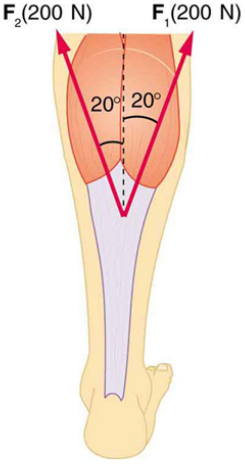
\includegraphics[width=0.15\textwidth]{figures/tendon.png}
\caption{\label{fig:tendon} Two muscles pull on the achilles tendon.}
\end{figure}
\item Consider an object on an inclined surface.  The object does not slide down the surface due to static friction. (a) Draw the free-body diagram, including all relevant forces.  (b) Show that if $\theta$ is the angle between the surface and horizontal, the coefficient of static friction is equal to $\tan\theta$. \\ \vspace{3cm}
\item Consider the drag coefficient from Fig. \ref{fig:drag}. (a) What is the force of drag on a Toyota Camry moving through air with $\rho_{air} = 1.225$ kg/m$^3$, cross-sectional area $A=4$ m$^2$, moving at $v=10$ m/s? (b) What happens to the drag force if the speed increases to $v=30$ m/s? \\ \vspace{2cm}
\begin{figure}
\centering
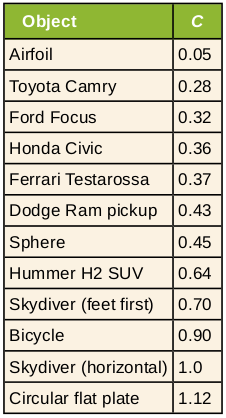
\includegraphics[width=0.15\textwidth]{figures/drag_table.png}
\caption{\label{fig:drag} Drag coefficients $C$ for various objects moving through air.}
\end{figure}
\end{enumerate}
\section{Rotational Motion and The Law of Gravity}
\begin{enumerate}
\item Condider Fig. \ref{fig:orbits}, depicting the orbits of the planets.  (a) Assume that Earth has an orbital period of 1.0 year, and an orbital radius of 1.0 AU.  The orbital period of Mars is observed to be about 1.88 years.  How far from the Sun is Mars (in AU)? (b) The orbital period of Jupiter is about 11.1 years.  How far is it from the Sun (in AU)? \\ \vspace{1.5 cm}
\begin{figure}[hb]
\centering
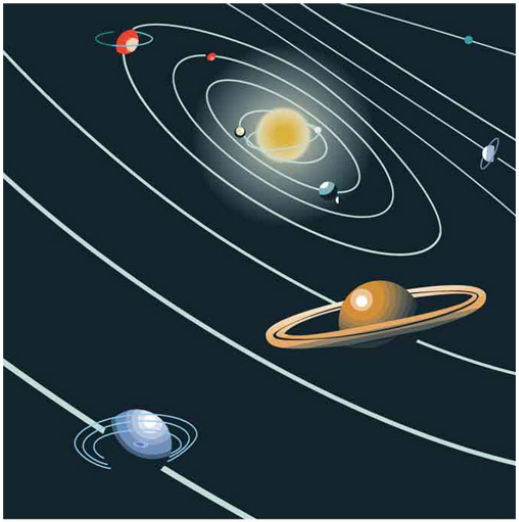
\includegraphics[width=0.2\textwidth]{figures/orbits.png}
\caption{\label{fig:orbits} The orbits of the planets obey Kepler's 3rd Law.}
\end{figure}
\item (a) What is the force of gravity between the Earth and the Sun?  Assume the mass of the Earth is $6\times 10^{24}$ kg, and the mass of the sun is $2\times 10^{30}$ kg. (b) In another star system, the masses of the planet and star are about the same as the Sun-Earth system, but the force is observed to be lower by a factor of nine. How far is the new planet from the new star? \\ \vspace{1.5cm}
\end{enumerate}
\section{Work, Energy and Momentum}
\begin{enumerate}
\item Two objects collide. Object 1 has mass $m_1 = 0.1$ kg, and object 2 has mass $m_2 = 0.2$ kg.  If the initial velocities are $v_1 = 10$ m/s and $v_2 = -10$ m/s, and the final velocity of object 1 is observed to be $v_1' = -20$ m/s, what is the final velocity of object 2, $v_2'$? \\ \vspace{2cm}
\item Suppose you are dragging a load with mass 50 kg across a surface that has a coefficient of friction of 0.05.  (a) If you drag the load for 10 meters, how much work have you done? (b) If you perform this task in 10 seconds, how much power are you consuming, in Watts?  (c) Sprinting apparently corresponds to 2400 Watts.  How does this compare to the power consumption in part (b)? \\ \vspace{2cm}
\end{enumerate}
\end{document}